\documentclass{article} % For LaTeX2e
\usepackage[final]{colm2025_conference}
\usepackage{graphicx}
\usepackage{amsmath}
\usepackage{microtype}
\usepackage{hyperref}
\usepackage{url}
\usepackage{booktabs}
\usepackage{lineno}
\usepackage{amsmath}
\usepackage{algpseudocode}
\usepackage{algorithm}
\usepackage{graphicx} % Required for inserting images
\usepackage{subcaption} % For subfigure arrangement
\usepackage{caption}
\usepackage{array}
\usepackage{booktabs}

\definecolor{darkblue}{rgb}{0, 0, 0.5}
\hypersetup{colorlinks=true, citecolor=darkblue, linkcolor=darkblue, urlcolor=darkblue}

\usepackage{etoolbox}
\makeatletter
\patchcmd{\@maketitle}
  {Published as a conference paper at COLM 2025}
  {}
  {}
  {}
\makeatother
\title{Week 8 Report}

% Authors must not appear in the submitted version. They should be hidden
% as long as the \colmfinalcopy macro remains commented out below.
% Non-anonymous submissions will be rejected without review.

\author{Mu Junrong}

% The \author macro works with any number of authors. There are two commands
% used to separate the names and addresses of multiple authors: \And and \AND.
%
% Using \And between authors leaves it to \LaTeX{} to determine where to break
% the lines. Using \AND forces a linebreak at that point. So, if \LaTeX{}
% puts 3 of 4 authors names on the first line, and the last on the second
% line, try using \AND instead of \And before the third author name.

\newcommand{\fix}{\marginpar{FIX}}
\newcommand{\new}{\marginpar{NEW}}

\begin{document}

\ifcolmsubmission
\linenumbers
\fi

\maketitle

\begin{abstract}
This report focuses on the training process and findings of the small transformer-based language model using the nanoGPT framework. The report explains the training loop in detail, including the model architecture and training loop. The training and validation curves are plotted to analyse the learning progress over time. Inference was performed using a modified \texttt{sample.py} script, generating continuations from given prompts.Inference is done and the outputs were compared the trained model from Week 7 report, and the causes of the difference are explained.
\end{abstract}

\section{Introduction to nanoGPT}
Currently, large language models (LLMs) are designed based on the Transformer architecture. The GPT (Generative Pre-trained Transformer) models (i.e., which includes only the decoder stack), originally introduced by OpenAI, has demonstrated strong capabilities in text generation, completion, summarization, and various other language tasks. However, training these models from scratch can be complex.

To simplify the process, nanoGPT was designed by Andrej Karpathy (\cite{nanoGPT}). nanoGPT is a minimal, streamlined, and efficient implementation of the GPT architecture in PyTorch. It focuses on code clarity and performance, offering a relatively small codebase that can train models on modest hardware with a few million parameters. nanoGPT is capable of training functioning generative models on character-level or tokenized datasets.

\subsection{nanoGPT architecture}
nanoGPT implements the standard decoder-only Transformer model (\cite{vaswani2017attention}). The model consists of the following key components:
\begin{itemize}
    \item Embedding Layer: Converts token IDs into dense vectors.
    \item Multiple Transformer Blocks: Each block includes multi-head self-attention, feed-forward networks (MLPs), layer normalisation, and residual connections.
    \item Output Head: A linear projection from hidden states to vocabulary logits for next-token prediction.
\end{itemize}
In the training process, the model is initialised with 12 layers, 12 attention heads, 768-dimensional embeddings and a block size of 1024 tokens per sequence.

These settings roughly correspond to the configuration of the original GPT-2 small (124M) model.

\subsection{Dataset: Shakespeare dataset}
For the training experiment, the Shakespeare dataset was used, which is a character-level corpus composed of lines from Shakespearean plays. The dataset is small in size but sufficient for training nanoGPT, that can learn to mimic Shakespearean style and structure at the character level. Each character is treated as a token, and sequences of characters are learned in an autoregressive manner.


\section{Training process of nanoGPT}

\subsection{Training loop}
The script \texttt{train.py} is the main training step of nanoGPT (\cite{nanoGPT}), and it supports both single-GPU training and Multi-GPU distributed training using Distributed Data Parallel (DDP). It mainly does the following:
\begin{itemize}
    \item initialises the model's configuration: number of layers, embedding and heads; checks if Distributed Data Parallel (DDP) is active; Enables TensorFloat32 for faster matmuls on Ampere+ GPUs
    \item \texttt{get\_batch(split)}: load data set, and returns x: input tokens and y: target tokens (i.e., next token prediction)
    \item \texttt{estimate\_loss()}: runs multiple batches through the model and returns average loss. It is Used to log metrics and save checkpoints
    \item \texttt{get\_lr(it)}: Implements cosine decay with warmup
    \item training loop: the loop is run until \texttt{max\_iters = 600000}. The training loop mainly fetches a new batch of input/output tokens, runs the model forward to compute loss, does backpropagate gradients to update model weights and log progress.

 \end{itemize}

\subsection{Training model and architecture}
nanoGPT follows the classic Transformer Decoder architecture with token and position embeddings and multiple transformer blocks (i.e., LayerNorm, masked multi-head self-Attention, MLP with GELU). The code \texttt{model.py} is the main model block for nanoGPT, and it mainly does the following:
\begin{itemize}
    \item \texttt{CausalSelfAttention}: implements masked multi-head self-attention. It projects the input into Q, K, V (i.e., query, key, value), computes attention, applies dropout and combines heads and projects the result back to the original dimension
    \item \texttt{MLP(nn.Module)}: Implements a standard 2-layer feedforward network with Gaussian Error Linear Unit (GELU) activation:
    \[
    \text{MLP}(x) = \text{Dropout}({W}_2(\text{GELU}({W}_1x + {b}_1)) + {b}_2)
    \]. It expands the dimension by 4 and projects back by x $\rightarrow$ Linear (expand) $\rightarrow$ GELU $\rightarrow$ Linear (compress) $\rightarrow$ Dropout.
    \item \texttt{forward (self, idx, targets=None)}: implements forward passing. 
    \item \texttt{F.cross\_entropy(logits.view($-1$, logits.size($-1$)), targets.view($-1$))
    }: calculates cross\-entropy which is the standard token-level loss which predicts the next token in sequence.

\end{itemize}


\section{Analysis of the results}
To examine the performance of nanoGPT, NVIDIA GPU and Python 3.9 are used. 
\subsection{Training and validation loss curves}
After the experiment, the training and validation loss curves are plotted using the logs recorded during training. 
\begin{figure}[H]
    \centering
      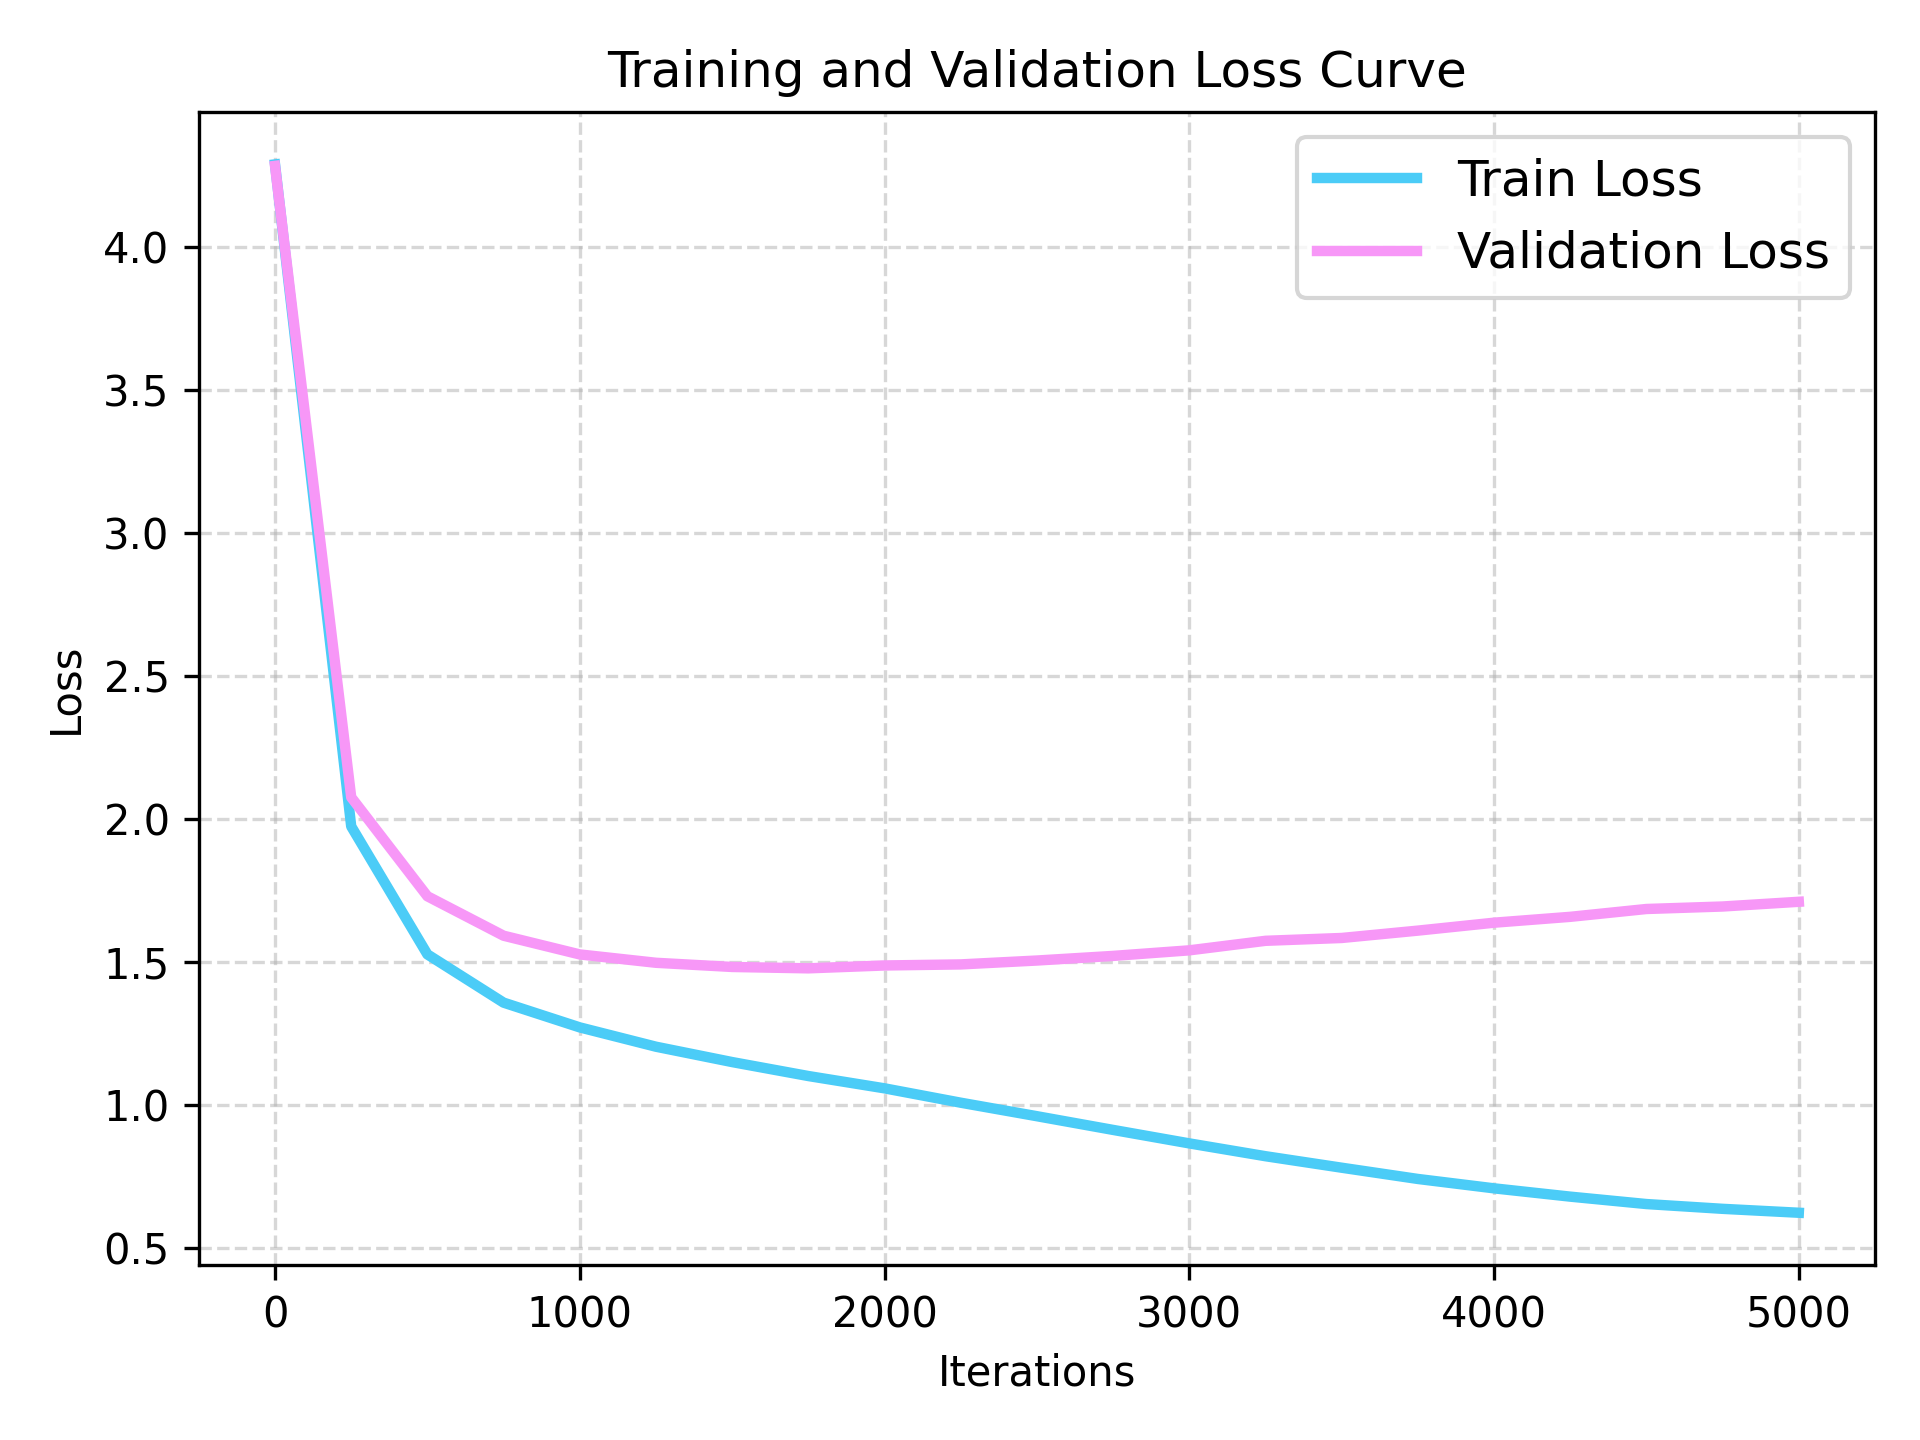
\includegraphics[width=1\linewidth]{loss_curve.png}
    \caption{Training and validation losses over time of the experiment}
    \label{fig:enter-label}
\end{figure}

\subsection{Analysis of the results}
Training loss measures the performance of the model on the training dataset (i.e., the data it sees and learns from during training). It is computed by comparing the model's predictions to the actual next tokens in the training set. The goal of training is to minimize this loss using optimization algorithms.

On the other hand, validation loss measures the performance of the model on unseen data which is not used for training (i.e., the validation dataset). It shows how the model's generalisation ability.

Both losses are calculated using Cross-entropy (\cite{goodfellow2016deep})
\[
Loss = -\sum_{i=1}^{|V|} y_i \log(p_i)
\]
where \( y_i \) is the true distribution (i.e., a one-hot vector; 1 for the correct token, 0 for others), and \( p_i \) is the predicted probability of token \( i \).

As shown by the curves, the training loss decreases steadily as number of training iterations increases, indicating that the model is learning patterns in the training dataset. The validation loss also decreases initially and tracks the training loss closely, which suggests that the model has good generalsation ability, and is not significantly overfitting.

However, after a number of iterations (i.e., around 2500 iterations), the validation loss slightly increases while training loss continues to drop. This could indicate the model has reached its capacity or begun overfitting. 

Overall, the loss curves demonstrate that the model is able to learn meaningful representations from the dataset.

\section{Inference and case studies}
To examine the model's inference ability, same questions are asked for both Qwen models and nanoGPT. Qwen-2.5-Instruct model is used, with the less creative temperature (i.e., $temperature = 0$ and $temperature = 6$). The following prompts are used for both models:
\begin{itemize}
    \item “The capital of Singapore is”
    \item “Who are you?”
    \item “What is the range of output of tanh?”
\end{itemize}

\subsection{Output analysis}
For prompts that are more fact-based, such as "what is the range of the output of tanh", Qwen-2.5-Instruct gives clear analysis and the final answer is correctly stated (i.e., $(-1, 1)$). However, nanoGPT trained on the Shakespeare dataset gives incorrect and meaningless output (i.e., quotation from Shakespeare "GLOUCESTER: All indeed, then I would by my griefs, Where you have no more blazed to thy woes.") (\cite{nanoGPT-vs-Qwen}).

For prompts that are open-ended such as "Who are you", Qwen-2.5-Instruct produces the output "What is your purpose in life?" repetitively, which is wrong and has no significance. On the other hand, nanoGPT produces more peotry-styled output (i.e., "EXETER: I am a point of those prince, I cannot ling; Which you will have laid my life to any often."), which is a more relevant response to the prompt (\cite{radford2018improving}). 

In general, nanoGPT trained on the Shakespeare data set generally generates more Shakespearean and creative output, while responding incorrectly to factual prompts. It is also less coherent and grammatically weaker compared to Qwen-2.5-Instruct. 

\subsection{Difference analysis}
The difference is mainly caused by 
the model size, training data and fine-tuning process (\cite{radford2019language}).
\begin{table}[H]
  \centering
  \begin{tabular}{|p{3cm}|p{5cm}|p{5cm}|}
    \hline
    & nanoGPT& Qwen-2.5-Instruct\\ \hline
    Model size and capability& The models has 124 million parameters, which is relatively small& The model has billions of parameters, ensures its high performance\\ \hline
    Training data size and type& The model is trained on only Shakespearean plays, which is dialogue-heavy and ancient English style (i.e., 1600s English). For example, factual questions including "range of tanh" never appear in Shakespeare, thus the model is unable to answer unseen math/science queries correctly& The model is trained on diverse internet-scale corpus, including the web, code and instructions. The data set is more general, modern and multilingual\\ \hline
 Fine-tuning process& The model is trained from scratch, and there is no instruction tuning involved&The model is fine-tuned with human instructions, for helpful responses\\\hline
  \end{tabular}
  \caption{nanoGPT v.s. Qwen-2.5-Instruct}
  \label{tab:your_label}
\end{table}

\bibliography{colm2025_conference}
\bibliographystyle{colm2025_conference}


\end{document}
